% non contare la pagina del titolo
\pagenumbering{gobble}

% titolo
\thispagestyle{empty}

\mdseries{

\vspace*{-1.5cm}
\begin{center}
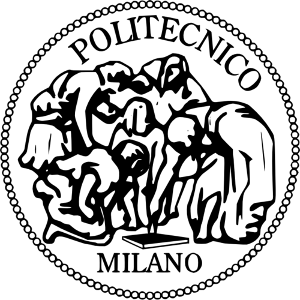
\includegraphics[width=5cm]{logo.png}

\vspace*{0.6cm}
{\LARGE\textsc{Politecnico di Milano}}\\
\rule{8.5cm}{1pt}

\vspace*{0.5cm}
{\large
Corso di Laurea Triennale in \textsc{Ingegneria Matematica}\\
Scuola di \textsc{Ingegneria Industriale e dell'Informazione}\\}

\vspace*{2.5cm} 
{\LARGE\textmd{\textbf{
The Cauchy-Kowalevski Theorem \\ 
\vspace*{2mm} 
and Its Consequences 
}}}
\vspace*{2.5cm} 

{\large
Thesis by
\vspace*{0.3cm}\\
Alessandro Pedone\\
Student ID 981105

\vspace*{1.75cm} 
Advisor:
\vspace*{0.3cm}
\\Prof. Maurizio Grasselli

\vfill
\rule{7.75cm}{1pt}

Graduation Session September 2024\\
\vspace*{1mm}
Academic Year 2023/2024}
\end{center} 
\clearpage
}
\blankpage


% conta con i numeri romani 
\pagenumbering{roman}

% citazione
\setlength\epigraphwidth{8cm}
\setlength\epigraphrule{0pt}
\vspace*{\fill}
\epigraph{\textit{All his life -- he had difficulty saying this, as he admitted, being always wary of too much enthusiasm -- all his life he had been waiting for such a student to come into this room. 
\\A student who would challenge him completely, who was not only capable of following the strivings of his own mind but perhaps of flying beyond them.}}{--- \textup{Alice Munro}, \textit{Too Much Happiness}}
\vspace*{\fill}

\newpage
\blankpage